\subsection{Endeligt koncept} \label{Endeligt koncept}
Det endelige konceptdesign fremgår af figur \ref{fig:skitse af endeligt koncept med navne}, hvor tre sæt af ledeskruer og følgestænger, danner bevægelsessystemet i henholdsvist to x-akser og én y akse.

\begin{figure}[H]
    \centering
    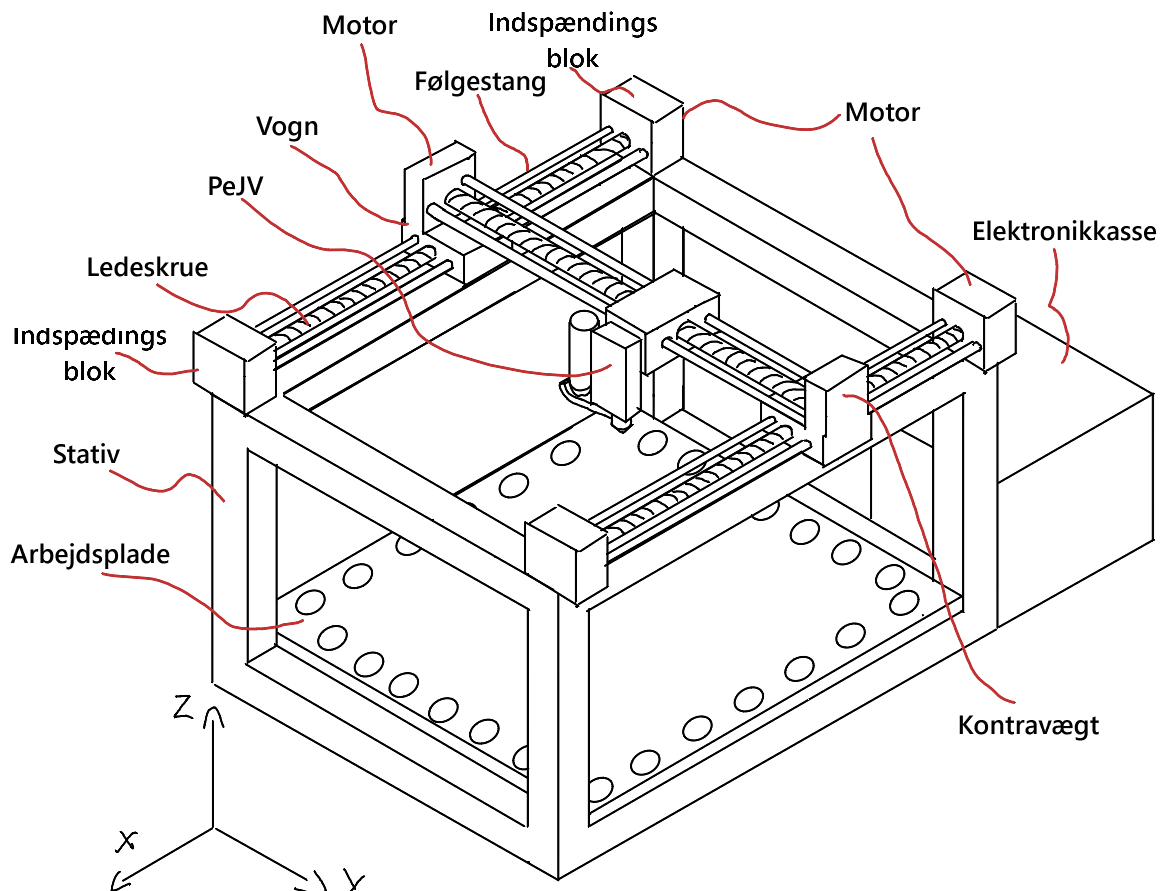
\includegraphics[width=0.7\linewidth]{Sections/6 Detaljeløsning/Media/Skitse med navne.png}
    \caption{Skitse af endeligt koncept med navne}
    \label{fig:skitse af endeligt koncept med navne}
\end{figure} \plainbreak{-.5}

Opsætningen er valgt med fokus på at sikre præcis lineær bevægelse af PeJV'en hen over emnet. I figuren ses, hvordan hovedet bevæger sig langs to parallelle følgestænger, hvor ledeskruen står for fremdriften. Denne mekaniske opsætning gør systemet stabilt, hvilket er nødvendigt for at opnå den påkrævede præcision.


